\documentclass[12 pt]{extarticle}

	\usepackage[frenchb]{babel}
	\usepackage[utf8]{inputenc}  
	\usepackage[T1]{fontenc}
	\usepackage{amssymb}
	\usepackage[mathscr]{euscript}
	\usepackage{stmaryrd}
	\usepackage{amsmath}
	\usepackage{tikz}
	\usepackage[all,cmtip]{xy}
	\usepackage{amsthm}
	\usepackage{varioref}
	\usepackage{pstricks-add, pst-plot}
\usepackage{auto-pst-pdf}
	\usepackage[margin=0.55in]{geometry}
	\geometry{a4paper}
	\usepackage{lmodern}
	\usepackage{hyperref}
	\usepackage{array}
	 \usepackage{fancyhdr}
	 \usepackage{float}
	\pagestyle{fancy}
	\theoremstyle{plain}
	\fancyhead[L]{Contrôle}
	\fancyfoot[C]{\emph{Tourner la page pour les questions}}
	\fancyhead[R]{9 décembre 2024}

	\title{Interrogation de calcul}
	\date{}
	\begin{document}

\begin{center}{\Large Contrôle de calcul}\\
 \end{center} 
 \subsection*{Exercice 1 (8 points)}
   \begin{enumerate}
   \item Réduire : $(-5x)^3$
   \item Réduire : $(4xy)(-3xz)(2z)$
   \item Réduire : $4-(6x+12)$
   \item Réduire : $-(8x-15)-6$
   \item Réduire : $(2x-3)-(x+1)$
   \item Développer et réduire : $(9x-8)(-6x+5)$
   \item Développer et réduire : $(2x+1)^2$
   \item Réduire : $4a^2-\frac23a - \frac35a^2+\frac13a-5a-\frac2{15}a^2$ \end{enumerate}


 \subsection*{Exercice 2 (6 points)}  
 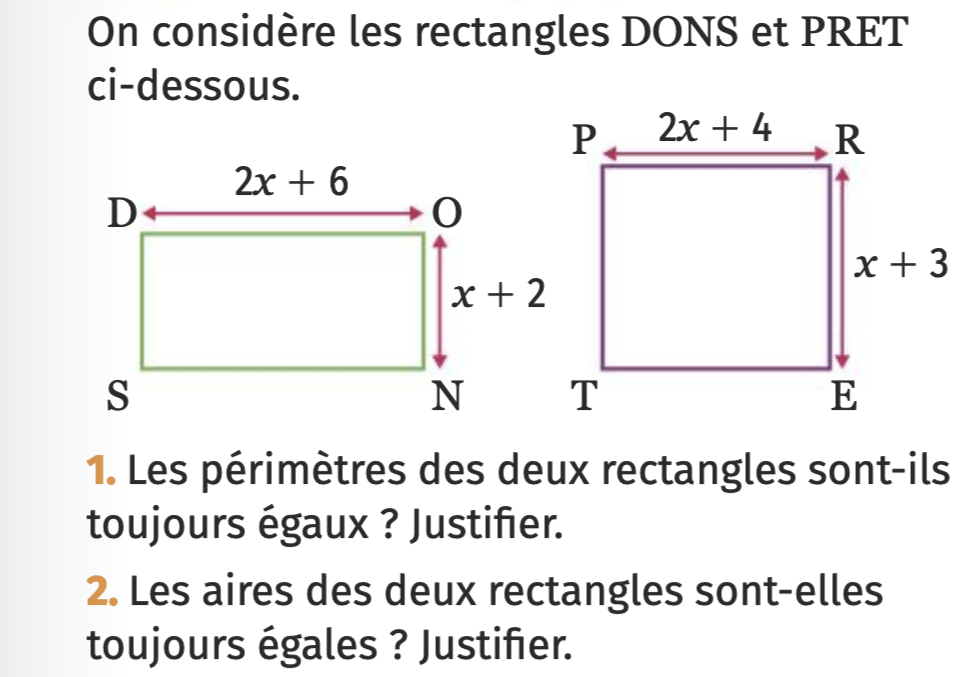
\includegraphics[scale=.65]{Exo2}
 \subsection*{Exercice 3 - DNB Nouvelle Polynésie  (6 points)}

On considère le programme de calcul suivant :
\begin{center}
 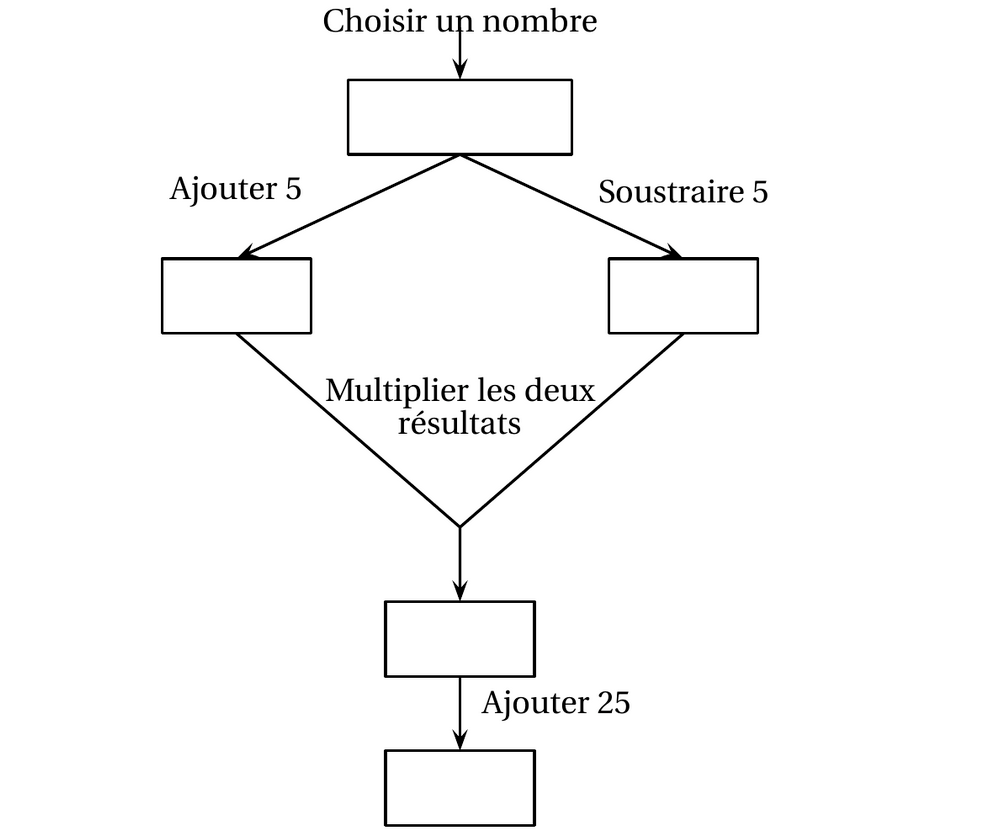
\includegraphics[scale=.5]{Exo3}

\end{center}
\begin{enumerate}
\item 
	\begin{enumerate}
		\item Si on choisit le nombre $7$, vérifier qu'on obtient 49 à la fin du programme
		\item Si on choisit le nombre $- 4$, quel résultat obtient-on à la fin du programme ?
	\end{enumerate}	
\item On note $x$ le nombre choisi au départ
	\begin{enumerate}
		\item Exprimer en fonction de $x$ le résultat obtenu. 
		\item Développer et réduire $(x + 5)(x - 5)$.
		\item Sarah dit : \og Avec ce programme de calcul, quel que soit le nombre choisi au départ, le résultat obtenu est toujours le carré du nombre de départ \fg.
		
Qu'en pensez-vous ?
	\end{enumerate}
\end{enumerate}

\subsection*{Bonus}
Développer et réduire : \[(2a+5b)(3a-2b)-(2a-1)(3a+2b)-(a-2b)(5b-1)\]
 	\end{document}
